
%%======%%======%0%======%%=======%%

\section{Materiais e métodos}
%\addcontentsline{toc}{chapter}{Objetivos}

%%======%%======%0%======%%=======%%
\subsection{Descrição do módulo}
A placa utilizada para a prototipagem e desenvolvimento do projeto, foi um módulo que integra um microcontrolador \textbf{ESP32}, equipado com um display LCD, e uma antena de LoRa (\textit{Long Range}). Além disso, o kit ainda contempla um sensor \textbf{Bosch BME 280}, o qual apresenta comunicação serial com o ESP32, via I2C  (\textit{Inter-Integrated
Circuit}) ou SPI (\textit{Serial Peripheral Interface}), e é capaz de analisar as seguintes variáveis:
\begin{itemize}
	\item pressão;
	\item temperatura;
	\item umidade;
	\item altitude.
\end{itemize}
O ESP32 utilizado, apresenta a seguinte configuração de \textit{pinout}:

\begin{figure}[H]
	\centering
	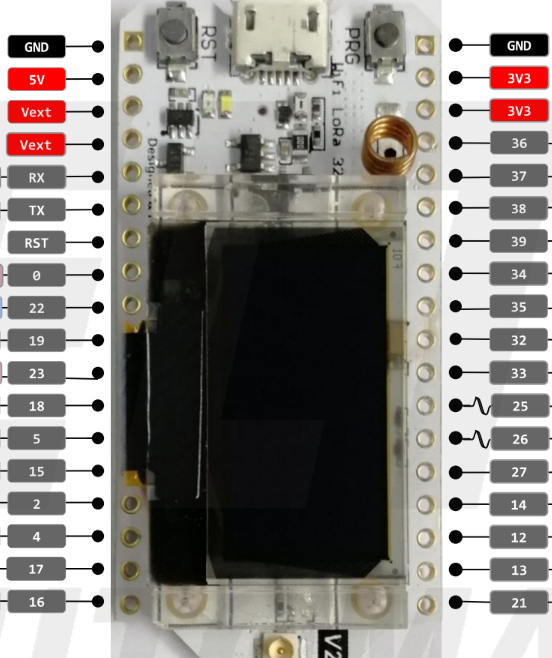
\includegraphics[width=0.4\linewidth]{2-imagens/pinout_esp}
	\caption{Fotografia do\textit{Pinout} da placa ESP32 LoRa.}
	\label{fig:pinoutesp}
\end{figure}
\begin{center}
	Fonte: \cite{heltec_wifi_lora_32_v2}, 2026.
\end{center}

